\begin{figure}[htbp]
    \centering
    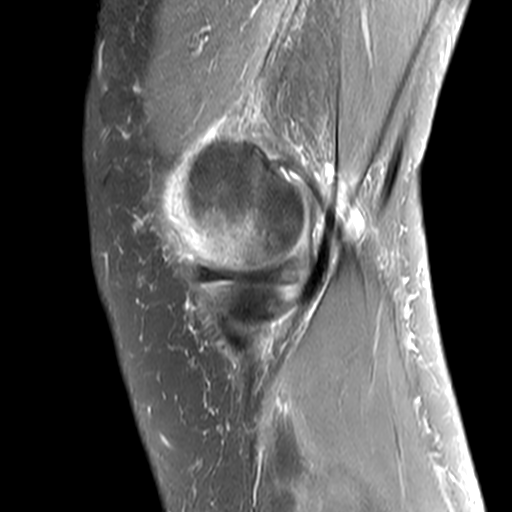
\includegraphics[width=\columnwidth]{corte_rodilla.png}
    \caption{Ejemplo de un corte sagital de resonancia magnética de rodilla
    del conjunto RSNA Knee Abnormality Detection. Se ajustó el contraste
    para visualización \cite{rsnadata}.}
    \label{fig:corte-rodilla}
\end{figure}

La Fig.~\ref{fig:corte-rodilla} muestra una sección del interior de la rodilla.
Esta imagen es uno de los cortes que componen una serie del estudio;
no representa por sí sola el examen completo ni confirma un hallazgo clínico.
